\documentclass[tikz,border=12pt]{standalone}
\usepackage[T1]{fontenc}
\usepackage{lmodern,amsmath,amssymb}
\usetikzlibrary{arrows.meta,positioning}
\definecolor{ink}{HTML}{183444}
\definecolor{blue}{HTML}{1B6780}
\definecolor{amber}{HTML}{AD601A}
\begin{document}
\hyphenpenalty=10000\exhyphenpenalty=10000
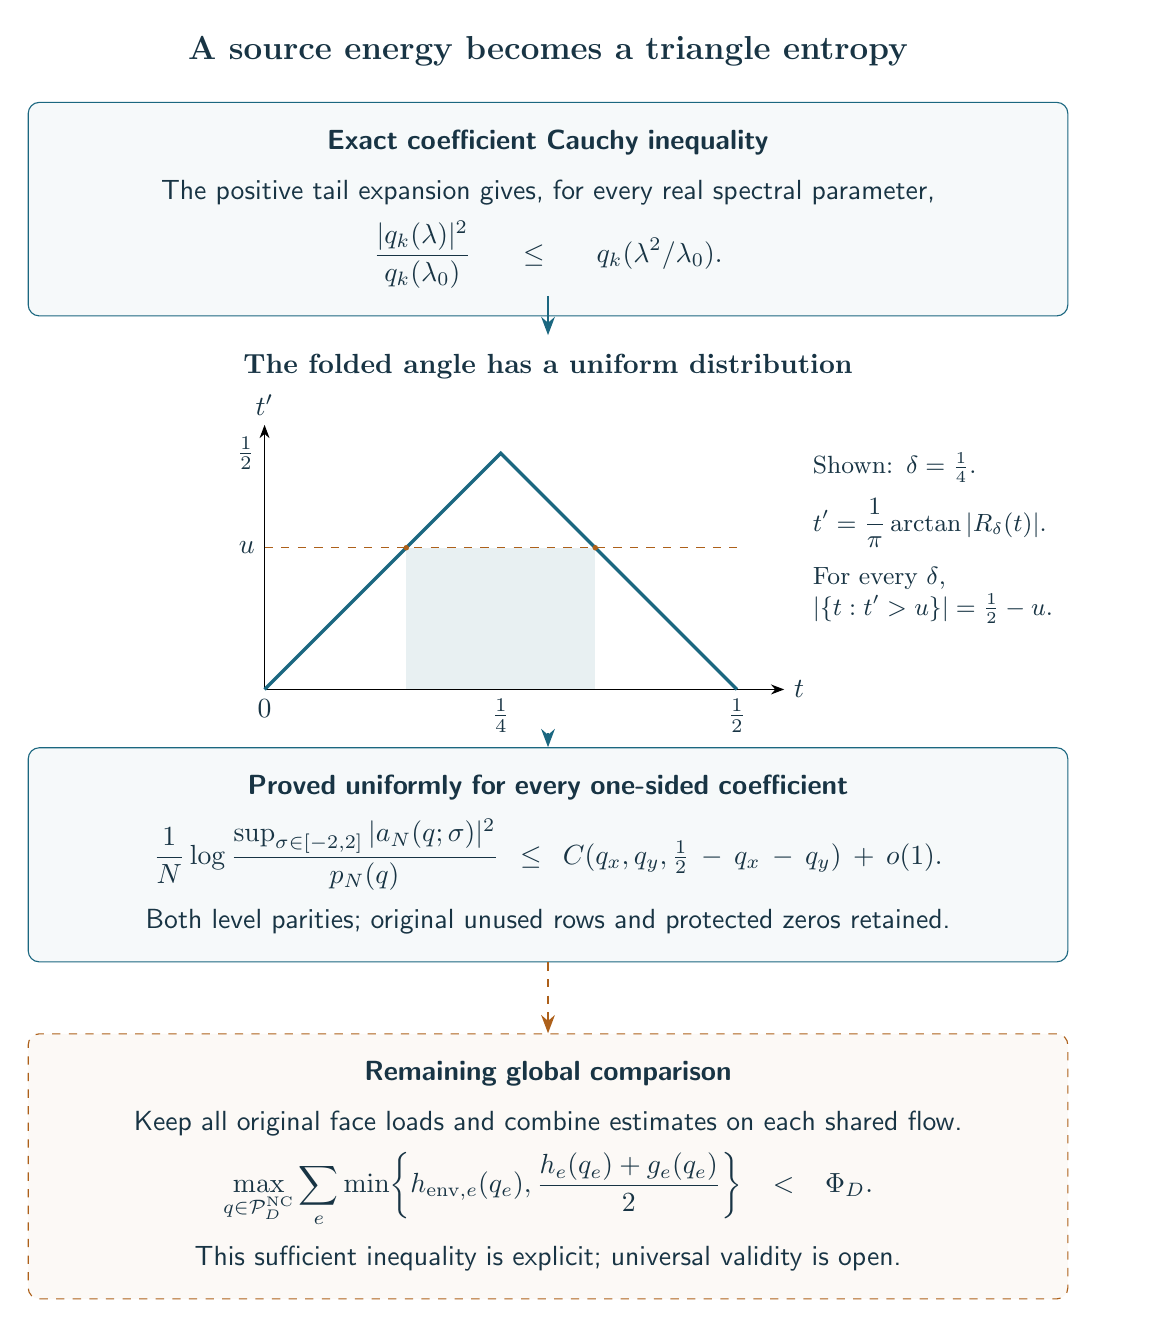
\begin{tikzpicture}[font=\sffamily,text=ink,>=Stealth,
 panel/.style={draw=blue,fill=blue!4,rounded corners,align=center,inner sep=10pt,text width=12.5cm},
 pending/.style={panel,draw=amber,fill=amber!4,dashed}]
\node[font=\large\bfseries] at (0,2.5) {A source energy becomes a triangle entropy};
\node[panel] at (0,.5) {\textbf{Exact coefficient Cauchy inequality}\\[6pt]
The positive tail expansion gives, for every real spectral parameter,\\[5pt]
$\displaystyle \frac{|q_k(\lambda)|^2}{q_k(\lambda_0)}
 \leq q_k(\lambda^2/\lambda_0).$};
\draw[->,thick,blue] (0,-.6)--(0,-1.1);
\node[font=\bfseries] at (0,-1.5) {The folded angle has a uniform distribution};
\begin{scope}[shift={(-3.6,-5.6)},x=12cm,y=6cm]
\fill[blue!10] (.15,0) rectangle (.35,.3);
\draw[->] (0,0)--(.55,0) node[right] {$t$};
\draw[->] (0,0)--(0,.56) node[above] {$t'$};
\draw[blue,very thick] (0,0)--(.25,.5)--(.5,0);
\draw[amber,dashed] (0,.3)--(.5,.3);
\fill[amber] (.15,.3) circle[radius=.35mm] (.35,.3) circle[radius=.35mm];
\node[below] at (0,0) {$0$};
\node[below] at (.25,0) {$\tfrac14$};
\node[below] at (.5,0) {$\tfrac12$};
\node[left] at (0,.3) {$u$};
\node[left] at (0,.5) {$\tfrac12$};
\node[align=left,anchor=west,text width=4cm,font=\small] at (.57,.32)
{Shown: $\delta=\tfrac14$.\\[5pt]
$\displaystyle t'=\frac1\pi\arctan|R_\delta(t)|$.\\[6pt]
For every $\delta$,\\
$|\{t:t'>u\}|=\tfrac12-u$.};
\end{scope}
\node[panel] (local) at (0,-7.7) {\textbf{Proved uniformly for every one-sided coefficient}\\[6pt]
$\displaystyle \frac1N\log\frac{\sup_{\sigma\in[-2,2]}|a_N(q;\sigma)|^2}{p_N(q)}
 \leq C(q_x,q_y,\tfrac12-q_x-q_y)+o(1).$\\[6pt]
Both level parities; original unused rows and protected zeros retained.};
\draw[->,thick,blue] (0,-6.15)--(local.north);
\node[pending,below=9mm of local] (global) {\textbf{Remaining global comparison}\\[6pt]
Keep all original face loads and combine estimates on each shared flow.\\[5pt]
$\displaystyle \max_{q\in\mathcal P_D^{\rm NC}}
  \sum_e\min\!\left\{h_{{\rm env},e}(q_e),
             \frac{h_e(q_e)+g_e(q_e)}2\right\}<\Phi_D.$\\[6pt]
This sufficient inequality is explicit; universal validity is open.};
\draw[->,thick,amber,dashed] (local)--(global);
\end{tikzpicture}
\end{document}
